\chapter{Conversion Service}

\section{Methodology}

The objective of the Conversion Service is to convert a given set of input WHIs into dzi files. Since a dzi is layered into a pyramid scheme, it is necessary to calculate the needed number of levels, as well as the dimensions of each level (see fig. 3.1 for an example).

\begin{figure}[H]
	\begin{center}
		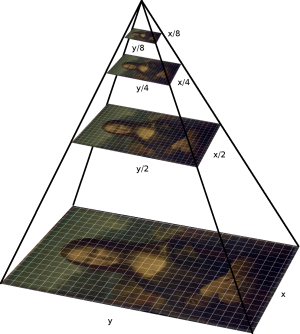
\includegraphics[scale=0.5]{img/pyramid.png}
		\caption{Example of a pyramid scheme in image processing (source: http://iipimage.sourceforge.net/images/pyramid.png)}
		\label{fig:fig3.1}
	\end{center}
\end{figure}

Therefore, the Conversion Service must be able to open an WHI $img_{input}$ of any of the in 2.2.1 defined formats. Based on the size of $img_{input}$ the number of necessary levels $lvl$ must be calculated. Once $lvl$ has been determined, $img_{input}$ must be resized into an appropriate scale for each $lvl_i$ in $lvl$. The resized image will be called $img_i$, with $i$ representing the corresponding level. In the next step, every $img_i$ will be tessellated into $x*y$ tiles. Each tile will be referrenced via $t^i_{c,r}$, with $r$ being the row and $c$ being the column of the tile in $whi_i$. To complete the conversion, the Conversion Service must create a describing xml file for each converted image $img_{dzi}$.


\subsection{Creating a Deep Zoom Image}

To create a dzi, the Conversion Service must be capable of all the afore mentioned tasks. According to \cite{web:openseadragon}, there is a number of frameworks, that can achieve this task (see tab. 3.1).

Since the conversion to dzi is required, two frameworks are not usable from the start. Those are MapTiler, who creates tms\footnote{Tile Map Service (tms) is a tile scheme developed and maintained by the Open Source Geospatial Foundation \cite{web:tms}} images and Kakadu, which creates iiif\footnote{International Image Interoperability Framework (iiif), specified by the International Image Interoperability Framework group, is an image delivery API which responds to requests via HTTP and HTTPS \cite{web:iiif}} images. Furthermore, the various desktop applications are not usable either, since the Conversion Service should operate as a microservice.

For ease of use and personal preferrence, the author settled with Deepzoom.py for the converison.\newpage

\begin{table}[H]
	\begin{center}
		\begin{tabular}{| p{3cm} | p{4cm} | p{2cm} |}
			\hline
			\textbf{option} & \textbf{description} & \textbf{image format} \\
			\hline
      		Deep Zoom Composer & dekstop app for Windows & dzi \\ \hline
      		Image Composite Editor & panoramic image stitcher from Microsoft Research for the Windows desktop & dzi \\ \hline
      		DeepZoomTools.dll & .NET-library, comes with Deep Zoom Composer & dzi \\ \hline
      		deepzoom.py & Python & dzi \\ \hline
      		deepzoom & Perl utility & dzi \\ \hline
      		PHP Deep Zoom Tools & PHP & dzi \\ \hline
      		Deepzoom & PHP & dzi \\ \hline
     		 DZT & an image slicing library and tool written in Ruby & dzi \\ \hline
     		MapTiler &  desktop app for Windows, Mac, Linux & tms \\ \hline
      		VIPS & command line tool and library for a number of languages & dzi (via dzsave feature) \\ \hline
     		Sharp & Node.js, uses VIPS & dzi \\ \hline
      		MagickSlicer & shell script (Linux/Max) & dzi \\ \hline
      		Gmap Uploader Tiler & C++ & dzi \\ \hline
      		Node.js Deep Zoom Tools & Node.js, under construction & dzi \\ \hline
      		OpenSeaDragon DZI Online Composer & Web app (and PERL and PHP scripts) & dzi \\ \hline
      		Zoomable & service, offers embeds; no explicit API & dzi \\ \hline
      		ZoomHub & service, under construction & dzi \\ \hline
      		Kakadu & C++ library to encode or decode JPEG 2000 images & iiif \\ \hline
      		PyramidIO & Java (command line and library) & dzi \\ \hline
  		\end{tabular}
  	\caption{Overview of conversion options for zooming image formats (source: \cite{web:openseadragon})}
  	\end{center}
\end{table}


\subsection{Deepzoom.py}

Deepzoom.py\footnote{see \url{https://github.com/openzoom/deepzoom.py} for further details} is a python script and part of Open Zoom\footnote{see \url{https://github.com/openzoom} for further details}. It can either be called directly over a terminal or imported as a module in another python script. The conversion procedure itself is analogous for both methods.

If run in a terminal the call looks like the following:

\begin{lstlisting}
	$ python deepzoom.py [options] [input file]
\end{lstlisting}

The various options and their default values can be seen in tab. 3.2. If called without a designated output destination, deepzoom.py will save the converted dzi right next to the original input file.

\begin{table}[H]
	\begin{center}
		\begin{tabular}{| r | l | r |}
			\hline
			\textbf{option} & \textbf{description} & \textbf{default} \\ \hline
			-h & show help dialog & - \\ \hline
			-d & output destination & - \\ \hline
			-s & size of the tiles in pixels & 254 \\ \hline
			-f & image format of the tiles & jpg\\ \hline
			-o & overlap of the tiles in pixels (0 - 10) & 1 \\ \hline
			-q & quality of the output image (0.0 - 1.0) & 0.8 \\ \hline
			-r & type of resize filter & antialias \\ \hline
		\end{tabular}
		\caption{Options for deepzoom.py}
	\end{center}
\end{table}

The resize filter is applied to interpolate the pixels of the image when changing its size for the different levels. Supported filters are:

\begin{itemize}
	\item cubic
	\item biliniear
	\item bicubic
	\item nearest
	\item antialias
\end{itemize}

When used as module in another python script, deepzoom.py can simply be imported via the usual \emph{import} command. To actually use deepzoom.py, a Deep Zoom Image Creator needs to be created. This class will manage the conversion process:

\begin{lstlisting}[frame=single]
# Create Deep Zoom Image Creator
creator = deepzoom.ImageCreator(tile_size=[size], 
	tile_overlap=[overlap],	tile_format=[format], 
	image_quality=[quality], resize_filter=[filter])
\end{lstlisting}

The options are analogous with the terminal version (compare tab. 3.2). To start the conversion process, the following call must be made within the python script:

\begin{lstlisting}[frame=single]
# Create Deep Zoom image pyramid from source
creator.create([source], [destination])
\end{lstlisting}

Upon calling, the ImageCreator opens the input image $img_{input}$ and creates a description with all the needed information for the dzis describing xml file\footnote{compare chap. 2.1.1}. After that, the number of levels is calculated. For this, the bigger value of height and width of $img_{input}$ is chosen (see eq. 3.1) and then used to determine the number of levels $lvl$ (see eq. 3.2).

\begin{equation}
	max{\textunderscore}dim = max(height, width)
\end{equation}

\begin{equation}
	lvl = {\lceil}log_2(max{\textunderscore}dim) + 1\rceil
\end{equation}

Once $lvl$ has been determined, $img_{input}$ will be resized in the chosen quality (-q/image{\textunderscore}quality) for every level $i$, with $i \in (0, lvl-1)$. The new resolution will be calculated for both dimensions $dim$ with a function $scale$ (see eq. 3.3) analogously. Furthermore, the image will be interpolated with the specified filter (-r/resize{\textunderscore}filter). The resized image will be called $img_i$.

\begin{equation}
	scale = {\lceil}dim * 0.5^{lvl-i}\rceil
\end{equation}

Once $img_i$ has been created, it will be tessellated into as many tiles of the specified size (-s/tile{\textunderscore}size) and with the specified overlap (-o/tile{\textunderscore}overlap) as possible. Since not every image will be of the size $2^n, n \in $ in either dimension, it is highly likely that the set of tiles for the last column/row will be smaller then specified in either dimension.

Every tile will be saved as [column]{\textunderscore}[row].[format] ([format] depending on -f/file{\textunderscore}format) in a folder called according to the corresponding level $i$. This folder will be located inside another folder, called [filename]{\textunderscore}files. The describing xml file will be persisted as [filename].dzi on the same level.


\section{Implementation}

As stated before, the Conversion Service is implemented as a python script. The script is to be called inside a terminal in the following fashion:

\begin{lstlisting}
	$ python ConversionService.py -i [folder]
\end{lstlisting}

There are two possible options for the call of ConversionService.py (see tab. 3.3), it's mandatory to pick one of the two, since there are no default values.

\begin{table} [h]
	\begin{center}
		\begin{tabular}{| r | l |}
			\hline
			\textbf{option} & \textbf{description} \\ \hline
			-h & show help \\ \hline
			-i & folder with WSI to convert \\ \hline
		\end{tabular}
		\caption{Options for ConversionService.py}
	\end{center}
\end{table}

Upon calling, the \emph{main()} routine will be started, which orchestrates the whole conversion process. It looks as follows:

\begin{lstlisting}[frame=single]
def main():
	path = checkParams()
	files = os.listdir(path)
	for file in files:
		print("-----------------------------------------")
		extLen = getFileExt(file)
		if(extLen != 0):
			print("converting " + file + "...")
			convert(path, file, extLen)
			print("done!")
\end{lstlisting}

\emph{checkParams()} will check if the input parameters are valid and, if so, return the path to the specified folder or exit otherwise. In the next step, the specified folder will be checked for its content. \emph{getFileExt(file)} looks up the extension of each given file and will either return the length of the files extension, if valid (\emph{extLen} $<0$) and $0$ otherwise. Each valid file will then be converted with the \emph{convert(...)} function:

\begin{lstlisting}[frame=single]
# convert image source into .dzi format
# param path: directory of param file
# param file: file to be converted
# param extLen: length of file extension
def convert(path, file, extLen):

	if not(path.endswith("/")):
		path += "/"
	dzi = file[:extLen] + "dzi"
	
	# create Deep Zoom Image creator
	creator = deepzoom.ImageCreator(tile_size=256, tile_overlap=0,
				tile_format="png", image_quality=1.0, 
				resize_filter="bicubic")

	# create Deep Zoom image pyramid from source
	creator.create(path + file, OUTPUT + dzi)
\end{lstlisting}

The name for the new dzi file will be created from the original file name, however, the former extension will be replaced by "dzi" (see line 9). Next, deepzooms ImageCreator will be initialized with the following parameters: tile{\textunderscore}size = 256, tile{\textunderscore}overlap = 0, tile{\textunderscore}format = "png", image{\textunderscore}quality = 1.0, resize{\textunderscore}filter = "bicubic" (see line 12 - 14). Once the ImageCreator is initialized, its \emph{create(...)} function is called (see line 17), in which the input image will be converted. The output will be saved to the same folder as ConversionService.py is operating from, plus "/dzi/".


\section{Test}

To test the correct functionality of the Conversion Service, an automated test will be deployed. The test will be in the form of a bash script (ConversionTest.sh), which calls ConversionService.py in a controlled evironment with a specific set of WSIs dedicated for testing purposes and verifies that the conversion succeeded.


\subsection{Setup}

The only requirement for this test is that a specified test directory (\emph{imgTest}, the test itself (\emph{ConversionTest.sh}) and \emph{ConversionService.py} are located in the same directory. 

If called, the conversion test will create a specific folder (\emph{csTest}), in which the testing will be done. Furthermore, a set of images from imgTest will be copied into the same folder. Afterwards, ConversionService.py is called, with \emph{imgTest/} as input directory. After ConversionService.py is done, the test will check if the output directory was created, as well as every image was converted successfully. The test can be considered a success, if both cases are given.


\subsection{Result}
